\begin{figure*}[t]
\centering
% src: fig/abc_fsc.png by scripts/paper_figures_abc.py; curves: docs/paper/fig_abc_fsc.csv; crossings: docs/paper/fig_abc_provenance.json (fsc_crossings_A)
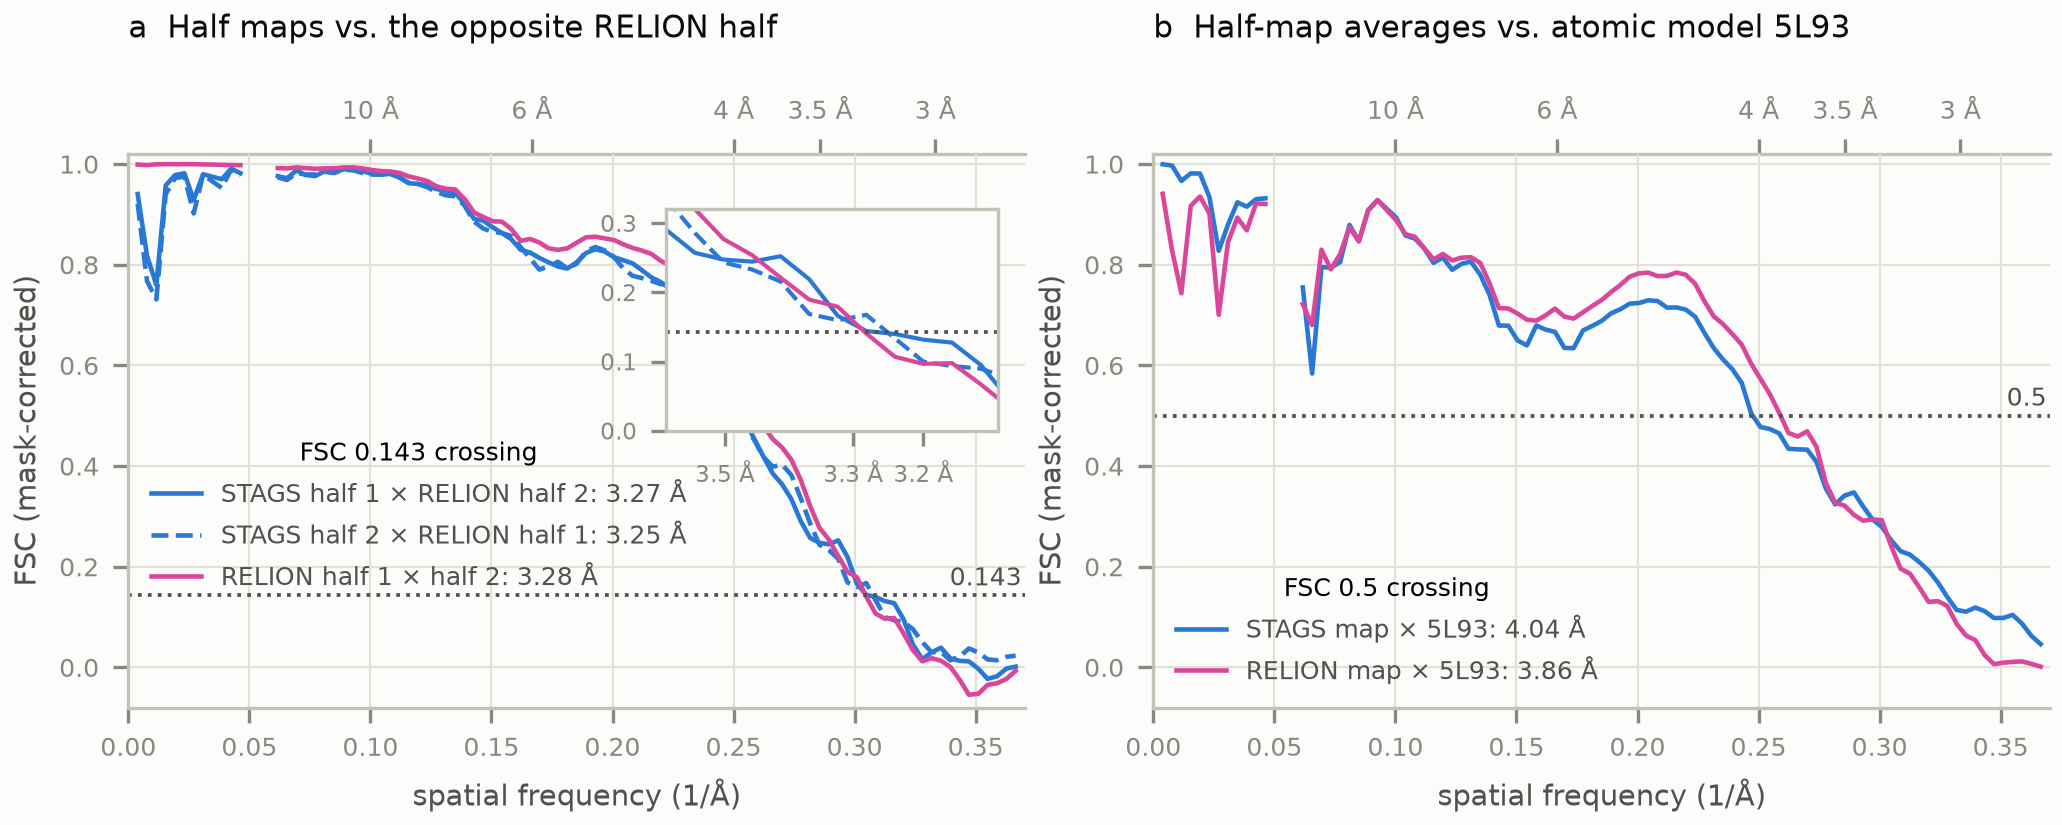
\includegraphics[width=\textwidth]{fig/abc_fsc.png}
\caption{\textbf{Fourier shell correlation, STAGS versus the RELION-5 polished map.}
(a)~Each STAGS half map against the opposite RELION-5 half map (blue; 3.27 and 3.25\,\AA\ at FSC~0.143) and RELION's own half 1 against half 2 (magenta; 3.28\,\AA); inset, 3.6--3.1\,\AA.
(b)~Average of the two normalized half maps against the atomic model 5L93: STAGS 4.04\,\AA, RELION-5 3.86\,\AA\ at FSC~0.5.
All curves: maps registered on RELION's $192^3$, 1.35\,\AA\ grid, RELION's mask, phase-randomization correction beyond 20\,\AA; gaps near 20\,\AA\ are the correction's transition shells, which the scorer leaves undefined.}
\label{fig:fsc}
\end{figure*}
